\section{FileSystemSecurity}
\subsection{Files permissions}
Chaque user a un UID et chaque group un GID. Les lists sont \verb!/etc/passwd! et \verb!/etc/group!. Il y a 3 types de permissions: read access (r), write access (2) et execute (access). Et c'est défini pour 3 type de user: owner,group,others (9bits: 3x rwx).
\begin{figure}[H]
\centering
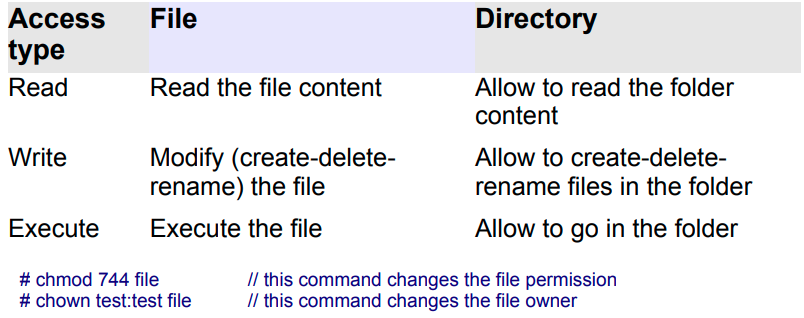
\includegraphics[width=0.9\columnwidth]{Figures/security_01.png}
\end{figure}
SUID or setuid: change user id on execution to owner (-rws on owner). SGID or setgid: change group ID on execution. Sticky bit: 2 fonctions, 1) process stay in memory after it finished et 2) a directory avec sticky bit permet de supprimer un fichier si on est le file owner (ça sert dans \verb!/tmp! on run). Pour mettre un le sticky bit on fait chmod 4755

\subsection{Contrôler et sécuriser les comptes}
Pour créer un user: \verb!adduser mdp! de base c'est du md5 mais on peut configurer pour que ça soit du sha512. Pour changer un mdp: \verb!passwd -a sha512 test1!

\subsection{Real and effective user id and group id}
Le user id réel c'est celui qu'on est \verb!whoami! et le effective c'est celui qu'on prendrait avec le suid.

\subsection{ACL}
Access control list qui permet de fine tune les droits dans un directory. Il faut l'ajouter dans make linux-menuconfig. Ext2, ext3, ext4, ReiserFS, JFS, XFS,
Btrfs, Tmpfs, JFFS2 et CIFS ont le ACL. On doit ajouter l'option au fstab lors du montage. Commande:
\begin{Verbatim}[breaklines=true, breakanywhere=true]
setfacl -m permissions fileOrDirectory
# example
setfacl -m u::rwx,g::r--,o:--- test // is equal to: chmod 740 test
# delete acl
setfacl -b test
# voir acl
getfacl TestDirectory/
\end{Verbatim}

\subsection{Attributs des fs ext2-4}
\begin{Verbatim}[breaklines=true, breakanywhere=true]
#set
chattr -i file
#get
lsattr file
\end{Verbatim}
Attributs: -i (peut pas être modifié, supprimé, renommé or lié même pas par le root), -A (date of access is not updated), -S (synchronous), -a (only in append mode), -c (auto compress), -d (not saved by the dump), -j (write to journal before data) et -s (quand le file est destroy, toutes les datas vont à 0)
\subsection{Rechercher les permissions de fichier faibles}
\begin{Verbatim}[breaklines=true, breakanywhere=true]
#file permissions = 200
find . -perm 200
#rechercher/retirer le setuid 
find / -type f -perm -4000 -ls 
chmod u-s /usr/bin/file 
chmod -R u-s /var/directory/ // Be careful
\end{Verbatim}

\subsection{Sécuriser les répertoires temporaires}
\verb!/tmp! ou \verb!/var/tmp! et une install classique linux va mettre le sticky bit (t) à la fin des perm sur tout le \verb!/tmp!. Une solution consiste à mettre ce \verb!/tmp! sur sa propre partition avec les options (nosuid, noexec, nodev (no node file), rw). Ensuite on peut supprimer le \verb!/var/tmp! et faire un lien symbolique qui pointe sur \verb!/tmp!. On peut aussi prendre un fs de type tmps fs pour \verb!/tmp! et tout avoir en ram.
Sinon on peut faire du loopback en créant un fichier de 1GB
\begin{Verbatim}[breaklines=true, breakanywhere=true]
dd if=/dev/zero of=/.tmpfs bs=1024 count=1000000
mkfs.ext4 /.tmpfs
mkdir /tmp
mount -o loop,noexec,nosuid,nodev,rw /.tmpfs /tmp
chmod 1777 /tmp
\end{Verbatim}
et faut ensuite ajouter dans fstab
\begin{Verbatim}[breaklines=true, breakanywhere=true]
/.tmpfs /tmp ext4 loop,nosuid,noexec,nodev,rw 0 0
\end{Verbatim}

\subsection{Mémorisation des mots de passe sous Linux}
Pour voir les mots de passes: \verb!cat /etc/shadow!
\begin{Verbatim}[breaklines=true, breakanywhere=true]
userame:$6(sha512)ou 1 (md5)$saltvalue$passwordCrypt:lastchanged(days since01.01.1970):4:5:6(number of days between password change)
\end{Verbatim}

\subsection{Casser un mot de passe}
5 types: Dictionary (file with words: a dictionary), Combinator (use 2 dict), Hybrid (dict + some letters), Brute force (try every combination) et Mask (brute force with inputs).

\subsection{Hashcat}
Rapide (peut être dans GPU)
\begin{Verbatim}[breaklines=true, breakanywhere=true]
#Summary: -m 0 à MD5
#Straight
hashcat -a 0 -m 0 hashfile dictionaryFile
#Combinator
hashcat -a 1 -m 0 hashfile dictionaryFile1 dictionaryFile2
#Brute force, mask
hashcat -a 3 -m 0 hashfile ?d?d?d
#Hybrid
hashcat -a 6 -m 0 hashfile ?u?u dictionaryFile ?d?d?d
# nanopi ex dict
hashcat -a 0 -m 500 h_test1.txt rockyou.txt
# nanopi brute force (le hash est dans h_test2.txt qui est la ligne de shadow)
hashcat -a 3 -m 500 h_test2.txt A?l?s?s3?l6S4
\end{Verbatim}
